\documentclass[a4paper,11pt]{article}
\input{/home/tof/Documents/Cozy/latex-include/preambule_doc.tex}
\input{/home/tof/Documents/Cozy/latex-include/preambule_commun.tex}
\newcommand{\showprof}{show them}  % comment this line if you don't want to see todo environment
\setlength{\fboxrule}{0.8pt}
\fancyhead[L]{\fbox{\Large{\textbf{Dicho 01}}}}
\fancyhead[C]{\textbf{Recherche dichotomique}}
\newdate{madate}{10}{09}{2020}
%\fancyhead[R]{\displaydate{madate}} %\today
\fancyhead[R]{Première - NSI}
\fancyfoot[L]{\vspace{1mm}Christophe Viroulaud}
\AtEndDocument{\label{lastpage}}
\fancyfoot[C]{\textbf{Page \thepage/\pageref{lastpage}}}
\fancyfoot[R]{\includegraphics[width=2cm,align=t]{/home/tof/Documents/Cozy/latex-include/cc.png}}
\usepackage{tikz}

\begin{document}
\section{Problématique}
Rechercher un élément dans un tableau est une opération courante. Cette tâche a un coût qui dépend de la taille du tableau.
% faire cas élément en début en fin au milieu
Cependant, si le tableau est déjà trié est-il possible d'accélérer la recherche?
\begin{center}
    \framebox{Comment implémenter une recherche efficace dans un tableau trié?}
\end{center}
\section{Recherche classique dans un tableau}
\subsection{Génération des données}
Imaginons un supermarché qui référence chaque article par un entier. Les références, au nombre de cent mille, sont contenues dans un tableau.
\begin{activite}
    Construire par compréhension un tableau de cent mille entiers compris entre 0 et 1000000.
\end{activite}
\subsection{Recherche dans les données}
Pour assigner une nouvelle référence, il faut d'abord vérifier que l'entier n'est pas déjà utilisé. Il faut parcourir le tableau élément par élément.
\begin{center}
    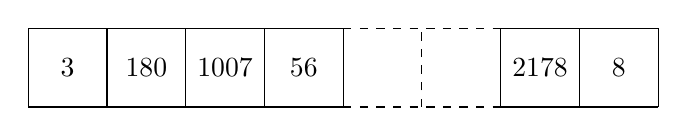
\begin{tikzpicture}
        \draw (0,0)grid(4,1);
        \draw[dashed] (4,0)grid(6,1);
        \draw (6,0)grid(8,1);
        \node at(0.5,0.5){3};
        \node at(1.5,0.5){180};
        \node at(2.5,0.5){1007};
        \node at(3.5,0.5){56};
        \node at(6.5,0.5){2178};
        \node at(7.5,0.5){8};


    \end{tikzpicture}
    \captionof{figure}{Parcours séquentiel}
\end{center}

\begin{aretenir}[]
Dans le pire des cas la complexité temporelle de la recherche dépend du nombre d'éléments.
\\
\centering La complexité temporelle est \textbf{linéaire}.
\end{aretenir}
% cas où l'élément n'est pas présent
\begin{activite}
    \begin{enumerate}
        \item Écrire la fonction \textbf{\texttt{recherche\_classique(tab: list, cherche: int) $\rightarrow$ bool}} qui renvoie \textbf{\texttt{True}} si l'entier \textbf{\texttt{cherche}} est présent dans le tableau.
        \item Tester la fonction: vérifier si le nombre 575000 est présent dans le tableau.
        \item Dans le programme principal, créer une variable \textbf{\texttt{COMPTEUR}} initialisée à 0. Cette variable de test sera utilisée \emph{dans la fonction} pour compter le nombre d'itérations de la boucle de recherche. On parle alors de \textbf{variable globale} car elle n'est pas propre à la fonction. Il faudra ajouter le code \ref{global} au début de la fonction.
        \begin{center}
        \begin{lstlisting}[language=Python  , xleftmargin=2em, xrightmargin=2em]
global COMPTEUR
\end{lstlisting}
        \captionof{code}{Déclaration d'une variable globale}
        \label{global}
        \end{center}
        % d'habitude pas préconisé
    \end{enumerate}
\end{activite}
\section{Recherche dans un tableau trié}
\subsection{Des données ordonnées}
Considérons maintenant que les références sont triées par ordre croissant au fur et à mesure de leur ajout dans le tableau de données.
\begin{center}
    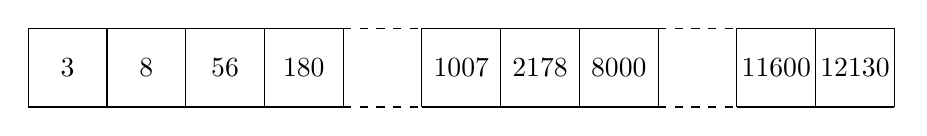
\begin{tikzpicture}
        \draw (0,0)grid(4,1);
        \draw[dashed] (4,0)grid(5,1);
        \draw (5,0)grid(8,1);
        \draw[dashed] (8,0)grid(9,1);
        \draw (9,0)grid(11,1);
        \node at(0.5,0.5){3};
        \node at(1.5,0.5){8};
        \node at(2.5,0.5){56};
        \node at(3.5,0.5){180};
        \node at(5.5,0.5){1007};
        \node at(6.5,0.5){2178};
        \node at(7.5,0.5){8000};
        \node at(9.5,0.5){11600};
        \node at(10.5,0.5){12130};
    \end{tikzpicture}
    \captionof{figure}{Références triées}
\end{center}
\begin{activite}
Pour simplifier nous allons utiliser la méthode \textbf{\texttt{sort}} pour trier les données.
\begin{enumerate}
    \item Construire par compréhension un tableau de cent mille entiers compris entre 0 et 1000000.
    \item Trier le tableau.
\end{enumerate}
\end{activite}
\subsection{Recherche dichotomique}
Les données étant triées, le principe de la dichotomie, pour chercher la présence d'un élément, consiste à:
\begin{itemize}
    \item couper le tableau en deux parties égales,
    \item ne garder que la partie contenant l'élément,
    \item répéter l'opération jusqu'à trouver l'élément ou avoir une partie vide.
\end{itemize}
Cherchons 302 dans le tableau suivant:
\begin{center}
    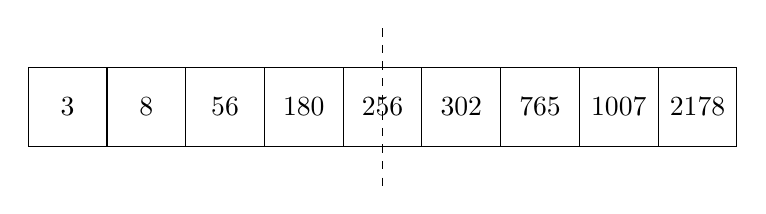
\begin{tikzpicture}
        \draw (0,0)grid(9,1);
        \node at(0.5,0.5){3};
        \node at(1.5,0.5){8};
        \node at(2.5,0.5){56};
        \node at(3.5,0.5){180};
        \node at(4.5,0.5){256};
        \node at(5.5,0.5){302};
        \node at(6.5,0.5){765};
        \node at(7.5,0.5){1007};
        \node at(8.5,0.5){2178};
        \draw[dashed] (4.5,1.5)--(4.5,-0.5);
    \end{tikzpicture}
    \captionof{figure}{Séparons les données en deux parties}
\end{center}
\begin{center}
    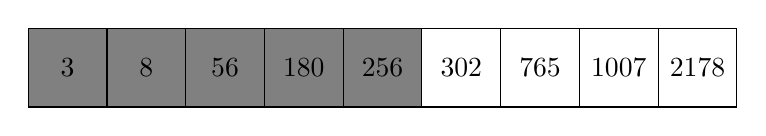
\begin{tikzpicture}
        \fill[gray] (0,0) -- (5,0) -- (5,1) -- (0,1)-- cycle;
        \draw (0,0)grid(9,1);
        \node at(0.5,0.5){3};
        \node at(1.5,0.5){8};
        \node at(2.5,0.5){56};
        \node at(3.5,0.5){180};
        \node at(4.5,0.5){256};
        \node at(5.5,0.5){302};
        \node at(6.5,0.5){765};
        \node at(7.5,0.5){1007};
        \node at(8.5,0.5){2178};
    \end{tikzpicture}
    \captionof{figure}{256 n'est pas le nombre recherché et il est inférieur à 302}
\end{center}
\begin{center}
    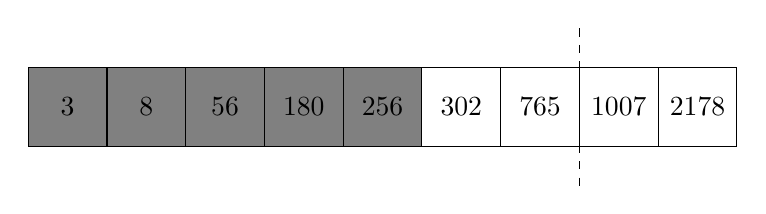
\begin{tikzpicture}
        \fill[gray] (0,0) -- (5,0) -- (5,1) -- (0,1)-- cycle;
        \draw (0,0)grid(9,1);
        \node at(0.5,0.5){3};
        \node at(1.5,0.5){8};
        \node at(2.5,0.5){56};
        \node at(3.5,0.5){180};
        \node at(4.5,0.5){256};
        \node at(5.5,0.5){302};
        \node at(6.5,0.5){765};
        \node at(7.5,0.5){1007};
        \node at(8.5,0.5){2178};
        \draw[dashed] (7,1.5)--(7,-0.5);
    \end{tikzpicture}
    \captionof{figure}{Séparons les données restantes en deux parties}
\end{center}
\begin{center}
    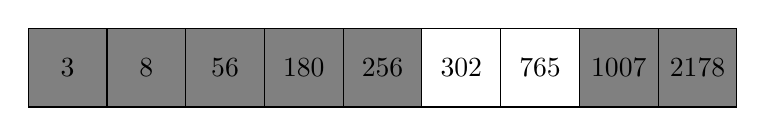
\begin{tikzpicture}
        \fill[gray] (0,0) -- (5,0) -- (5,1) -- (0,1)-- cycle;
        \fill[gray] (7,0) -- (9,0) -- (9,1) -- (7,1)-- cycle;
        \draw (0,0)grid(9,1);
        \node at(0.5,0.5){3};
        \node at(1.5,0.5){8};
        \node at(2.5,0.5){56};
        \node at(3.5,0.5){180};
        \node at(4.5,0.5){256};
        \node at(5.5,0.5){302};
        \node at(6.5,0.5){765};
        \node at(7.5,0.5){1007};
        \node at(8.5,0.5){2178};
    \end{tikzpicture}
    \captionof{figure}{Nous pouvons éliminer la partie supérieure à 302}
\end{center}
\begin{center}
    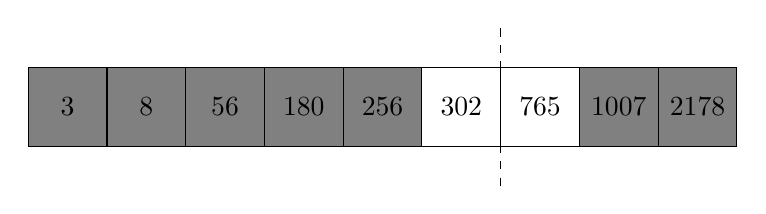
\begin{tikzpicture}
        \fill[gray] (0,0) -- (5,0) -- (5,1) -- (0,1)-- cycle;
        \fill[gray] (7,0) -- (9,0) -- (9,1) -- (7,1)-- cycle;
        \draw (0,0)grid(9,1);
        \node at(0.5,0.5){3};
        \node at(1.5,0.5){8};
        \node at(2.5,0.5){56};
        \node at(3.5,0.5){180};
        \node at(4.5,0.5){256};
        \node at(5.5,0.5){302};
        \node at(6.5,0.5){765};
        \node at(7.5,0.5){1007};
        \node at(8.5,0.5){2178};
        \draw[dashed] (6,1.5)--(6,-0.5);
    \end{tikzpicture}
    \captionof{figure}{Dernière séparation}
\end{center}
\begin{center}
    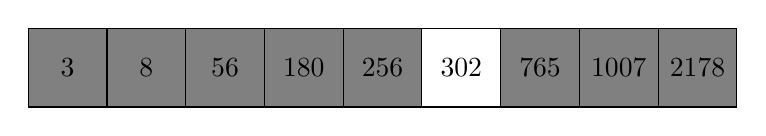
\begin{tikzpicture}
        \fill[gray] (0,0) -- (5,0) -- (5,1) -- (0,1)-- cycle;
        \fill[gray] (6,0) -- (9,0) -- (9,1) -- (6,1)-- cycle;
        \draw (0,0)grid(9,1);
        \node at(0.5,0.5){3};
        \node at(1.5,0.5){8};
        \node at(2.5,0.5){56};
        \node at(3.5,0.5){180};
        \node at(4.5,0.5){256};
        \node at(5.5,0.5){302};
        \node at(6.5,0.5){765};
        \node at(7.5,0.5){1007};
        \node at(8.5,0.5){2178};
    \end{tikzpicture}
    \captionof{figure}{302 a été trouvée en trois itérations}
\end{center}
\begin{activite}
Écrire la fonction \textbf{\texttt{recherche\_dicho(tab: list, cherche: int) $\rightarrow$ bool}} qui applique le principe de la dichotomie. Pour séparer les données en deux parties (à peu près) égales il faudra calculer l'indice médian de la partie encore valide.
\end{activite}
\subsection{Efficacité}
\begin{activite}
\begin{enumerate}
    \item En utilisant une variable \textbf{\texttt{COMPTEUR}}, compter le nombre d'itérations de la boucle de recherche dichotomique.
    \item Tester pour différentes tailles de tableau.
\end{enumerate}
\end{activite}
À chaque itération la quantité de données (notée \textbf{n}) à étudier est divisée par deux. Dans le pire des cas, on divise jusqu'à ce que la taille de la partie restante soit inférieure ou égale à 1.
% 0 = pas trouvé
$$\dfrac{n}{2^x}=1$$
$$\Leftrightarrow n=2^x$$
\begin{activite}
\begin{enumerate}
    \item Encadrer la valeur de \emph{x} entre deux entiers, si le tableau contient $n=10000$ éléments.
    \item Effectuer le même encadrement pour cent mille, un million d'éléments.
\end{enumerate}
\end{activite}
\begin{aretenir}[]
La complexité temporelle de la recherche dichotomique est \textbf{logarithmique}:
{\Large$$ \log_2{n} =x$$}
\end{aretenir}
\end{document}